\begin{figure}[th]
\centering
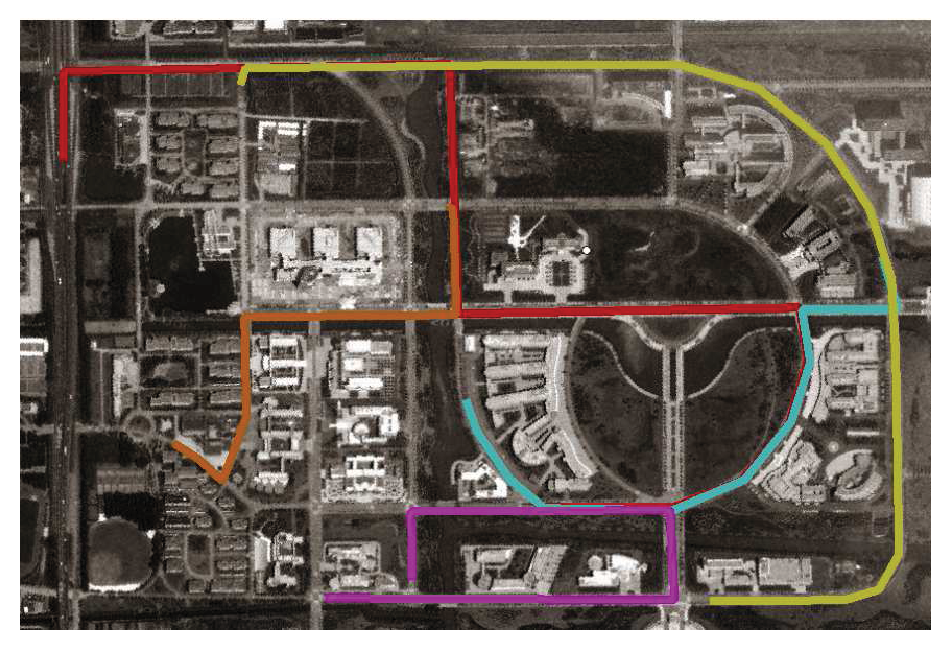
\epsfig{file=sjtu_trace.eps, width=0.7\columnwidth}
\caption{Five Inferred Traces on SJTU Campus}
\label{fig:sjtu}
\end{figure}

\begin{figure}
\begin{minipage}[th]{0.48\columnwidth}
\centering
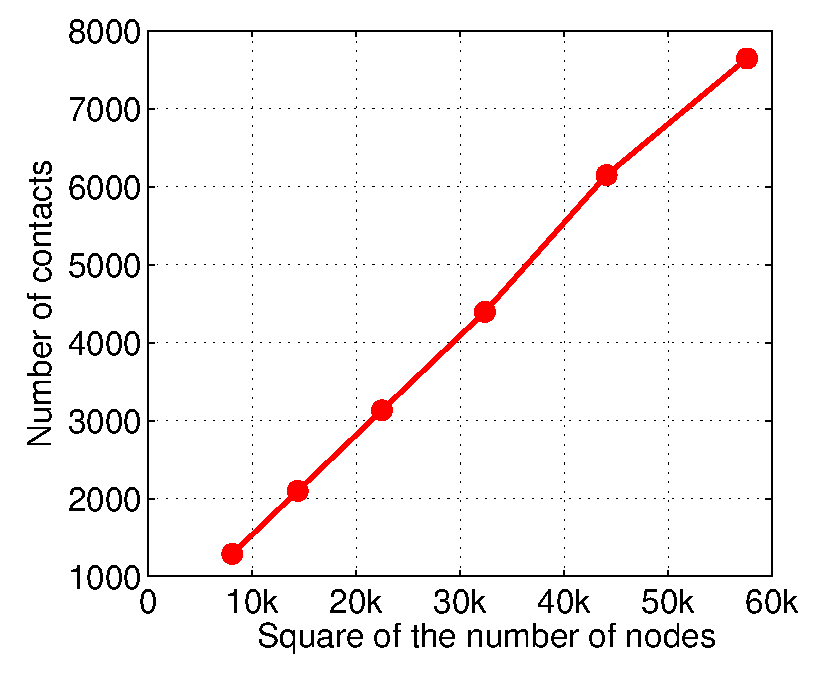
\epsfig{file=figure_n_c.eps, width=\columnwidth}
{\small(A)}
%\caption{Scale on Nodes}
%\label{fig:scale_nodes}
\end{minipage}
\hfill
\begin{minipage}[th]{0.48\columnwidth}
\centering
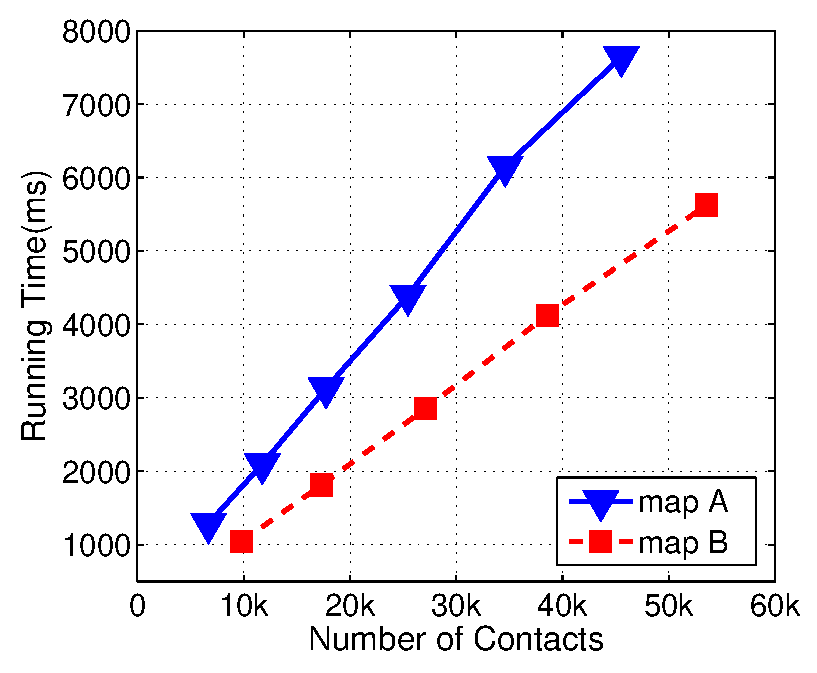
\epsfig{file=figure_scale.eps, width=\columnwidth}
{\small(B)}
\end{minipage}
\caption{Induced Contacts vs. Nodes (A)
Scale-up on Contacts (B)}
\label{fig:scale}
\end{figure}

\section{Preliminary Results}
We implement the approach, run it on numbers of synthetic data sets 
and get the following results. 
Each trace is generated by randomly selecting an origin
and a destination on a map of Shanghai Jiao Tong University
Campus and has a duration of 1 hour. Starting from the origin, we randomly
select the next location among all adjacent junctions. A junction 
is more likely to be selected if it is closer to the destination. 
From the traces, we can induce a list of contacts and their locations like the following:
\begin{center}
\fbox{
{\small
\begin{tabular}{ l  l  l  l  l  }
node0 & node2 & 339.7877 & 154.0384 & 17.5236\\
node0 & node2 & 41.2401 & 276.1339 & 87.4113\\
node0 & node179 & 41.3582 & 284.7934 & 92.3681\\
$\cdots$ & $\cdots$ & $\cdots$ & $\cdots$ &$ \cdots$
\end{tabular}
}
}
\end{center}
The columns represent the nodes in contact, the $X$ and $Y$ coordinates
of the contact location and contact time. The coordinates are
not used in inference but in validation.
We run 11 experiments and the sizes of contact histories range from hundreds to 60,000. 
All traces are correctly inferred.
Fig.\ref{fig:sjtu} shows 5 inferred trace fragments. Fig.\ref{fig:scale}(A) shows the number of contacts induced in the
data set is roughly proportional to the square of the number of nodes. 
Fig.\ref{fig:scale}(B) shows the running times of the
algorithm on various data sets. 
The solid line represents results for data on map $A$ 
with 48 junctions which corresponds to the area in Fig.\ref{fig:sjtu}. 
The dotted line represents the results for data on a smaller 
map $B$ with 25 junctions. 
The running time is almost linear to size of contact histories.
These preliminary results are in line with the discussion in Section \ref{sec:approach}.


